\documentclass{jsarticle}


\usepackage{ascmac}
\usepackage[top=30truemm,bottom=30truemm,left=25truemm,right=25truemm]{geometry}
\usepackage{amsfonts}
\usepackage{amsmath,amssymb}
\usepackage[dvipdfmx]{graphicx}
\usepackage{cases}

\begin{document}

\title{集合と位相}
\author{nukui}
\date{\today}
\maketitle

\part{集合と写像}
\section{集合とは}
\subsection{}
\begin{enumerate}
\item 成り立つ。$\because$ Yに含まれる要素は全てXに含まれる。
\item 成り立つ。$\because$3はWに含まれるがZに含まれない。
\item 成り立つ。$\because$4はVに含まれるが、Yに含まれない。
\item 成り立たない。$\because$4はVに含まれるがXには含まれない。
\item 成り立たない。$\because$ 1はXに含まれるがWに含まれない。
\item 成り立たない。$\because$ Vの全ての要素はWに含まれる。
\item 成り立つ。$\because$ Vの全ての要素はZに含まれる。
\item 成り立つ。 $\because$ 3はXに含まれるがZに含まれない。
\item 成り立たない。 $\because$ Yに含まれる全ての要素はZに含まれる。
\item 成り立たない。$\because$ 3はWに含まれるがYには含まれない。
\end{enumerate}

\subsection{}
\begin{enumerate}
\item D
\item B
\item C,E,F
\item B,D
\end{enumerate}

\subsection{}
\begin{enumerate}
\item 成り立たない。
\item 成り立つ。
\item 成り立つ。
\item 成り立つ。
\item 成り立たない。
\item 成り立つ。
\end{enumerate}

\subsection{}
集合Aが1個の元から成るとき、部分集合はAと$\emptyset$の2通り。よって$n=1$のとき、命題は成り立つ。\\
集合Aがn個の元から成り、その部分集合は全部で$2^n$個から成ると仮定する。
今、集合Aに元$X(X\notin A)$を一つ加え、$n+1$個の元から成る集合$B(B=A\cup\{X\})$を考える。
集合Bの部分集合は、
\begin{enumerate}
\item 集合Aの部分集合と一致。($2^n$個)
\item 集合Aの部分集合に元Xを加えたものに一致。($2^n$個)
\end{enumerate}
のいずれかである。よって、集合Bの部分集合の個数は$2^n+2^n=2^{n+1}$個になる。以上より、すべての自然数$n$で命題は成り立つ。

\section{集合の演算}
\subsection{}
意味を考えれば、確かに成り立つことがわかる。

\subsection{}
\begin{enumerate}
\item
\begin{align*}
(A-B)\cup(A\cap B)&=\{x|x\in(A-B) またはx\in(A\cap B)\}\\
&=\{x|(x\in A かつ x\notin B) または (x\in A かつ x\in B)\}\\
&=\{x|x\in A かつ (x\notin B または x\in B)\}\\
&=\{x|x\in A\}\\
&=A
\end{align*}


\item
\begin{align*}
(A-B)\cup B &=\{x| x\in (A-B) または x \in B\}\\
&=\{ x | (x \in A かつ x\notin B) または x\in B \}\\
&=\{x | (x\in Aまたは x\in B) かつ( x\notin B または x\in B)\}\\
&=\{x| (x\in Aまたは x\in B)\}\\
&=A\cup B
\end{align*}


\item
\begin{align*}
B\cap(A-B)&=\{x|x\in B かつ x \in(A-B)\}\\
&=\{x|x\in B かつ( x \in A かつ x\notin B)\}\\
&=\emptyset
\end{align*}
\end{enumerate}

\subsection{}
\begin{enumerate}
\item
$A_1 \subset A$を仮定する。
\[x \in A_1 かつ x\notin B \Longrightarrow x\in A かつ x\notin B\]
なので、$x\in A_1-B$とすると、$x\in A-B$が示せる。つまり、$A_1-B \subset A-B$。
\item
$B_1 \subset B$を仮定する。
\[x \in A かつ x\notin B \Longrightarrow x\in A かつ x\notin B_1\]
なので、$x\in A-B$とすると、$x\in A-B_1$が示せる。つまり、$A-B \subset A-B_1$。
\end{enumerate}

\subsection{}
\begin{align*}
A-B&=\{x|x\in A かつ x\notin B\}\\
&=\{x|x\in A かつ (x\notin A または x\notin B)\}\\
&=\{x|x\in A かつ x\notin A\cap B\}\\\\
A&=\{x|x\in A\}
\end{align*}
なので、
\[A-B=A \Longleftrightarrow  A-B \supset A \Longleftrightarrow A\cap B = \emptyset\]
となり、$A-B=A$と、$A\cap B=\emptyset$が同値であることを示せた。

\subsection{}
\begin{enumerate}
\item
定義から、
\begin{align*}
A\cup B &= \{x | x\in A または x\in B\}\\
B&= \{x| x\in B\}
\end{align*}である。
ここで、$A\subset B$を仮定すると、$A\cup B = \{x | x\in B\}=B$となる。逆に、$A\cup B= B$を仮定すると、$A\cup B \subset B$より、$\forall x [ x\in A \Longrightarrow x\in B]$となるので、$A\subset B$。\\

\item
定義から、
\begin{align*}
A\cap B &= \{x | x\in A かつ x\in B\}\\
A&= \{x| x\in A\}
\end{align*}である。
ここで、$A\subset B$を仮定すると、$A\cap B = \{x | x\in A\}=A$となる。逆に、$A\cap B= A$を仮定すると、$ A\cap B \supset A$より、$\forall x [ x\in A \Longrightarrow x\in B]$となるので、$A\subset B$。\\

\item 定義から
\[A-B=\{x|x\in A かつ x\notin B\}\]
である。ここで、$A\subset B$を仮定すると、$\forall x [ x\in A \Longrightarrow x\in B]$なので、$A-B=\emptyset$が成り立つ。逆に、$A-B=\emptyset$を仮定すると、$\forall x [ x\in A \Longrightarrow x\in B]$になるので、$A\subset B$が成り立つ。\\

\item 定義から
\begin{align*}
A\cup (B-A)&=\{x|x\in A または x\in (B-A)\}\\
&=\{x|x\in A または (x\in B かつ x\notin A)\}\\
&=\{x|x\in A または x\in B\}\\
&= A\cup B
\end{align*}
よって、1と本質的に同じ問題なので、成立する。\\
\item 定義から
\begin{align*}
B-(B-A)&=\{x| x\in B かつ x\notin (B-A)\}\\
&=\{x| x\in B かつ (x\notin B または x\in A)\}\\
&=\{x| x \in B かつ x\in A\}\\
&= A\cap B
\end{align*}
よって、本質的に2と同じ問題なので、成立する。
\end{enumerate}

\subsection{}
\begin{enumerate}
\item
\begin{align*}
(A\cup B) \cap (A\cup C) \cap(B\cup C) 
&=((A\cup B) \cap (A\cup C)) \cap(B\cup C) \\
&=((A\cup B) \cap A) \cup ((A\cup B) \cap C)) \cap(B\cup C) \\
&=(A\cup ((A\cap C) \cup (B\cap C)))\cap(B\cup C) \\
&=(A \cup (B\cap C))\cap(B\cup C) \\
&=(A\cap(B\cup C)) \cup ((B\cap C)\cap (B\cup C))\\
&=((A\cap B)\cup (A\cap C)) \cup (B\cap C)\\
&=(A\cap B)\cup (A\cap C) \cup (B\cap C)
\end{align*}
\item 1の結果を用いる。
\begin{align*}
&\quad(A\cup B) \cap (A\cup C) \cap(A\cup D)\cap (B\cup C) \cap (B\cup D) \cap(C\cup D)\\
&=((A\cup B) \cap (A\cup C)\cap(B\cup C) )\cap((A\cup D)\cap (B\cup D)\cap(C\cup D))\\
&=((A\cap B)\cup (A\cap C) \cup (B\cap C))\cap (D\cup (A\cap B \cap C))\\
&=(((A\cap B)\cup (A\cap C) \cup (B\cap C))\cap D)\cup(((A\cap B)\cup (A\cap C) \cup (B\cap C))\cap(A\cap B \cap C))\\
&=((A\cap B\cap D)\cup (A\cap C\cap D) \cup (B\cap C\cap D))\cup (A\cap B \cap C)\\
&=(A\cap B \cap C)\cup(A\cap B\cap D)\cup(A\cap C\cap D)\cup (B\cap C\cap D)
\end{align*}
\end{enumerate}


\section{ド・モルガンの法則}
\subsection{}
\begin{enumerate}
\item
\begin{align*}
(A^c)^c&=(X-A)^c\\
&=\{x | x\in X - (X-A)\}\\
&=\{x\in X|x \notin X-A\}\\
&=\{x\in X|「x \in X かつ x \notin A」ではない\}\\
&=\{x\in X| x\notin X または x \in A\}\\
&=\{x\in X | x \in A\}\\
&= A
\end{align*}


\item
\[X^c = X-X =\{x| x\in X かつ x\notin X\}= \emptyset \]

\item
\[\emptyset^c = X-\emptyset = \{x | x\in X かつ x\notin \emptyset\} = X\]

\item
\begin{align*}
A\cup A^c &= \{x| x\in A または x\in A^c\}\\
&=\{x \in X | x \in A または x\notin A\}\\
&=X
\end{align*}

\item
\[A\cap A^c = (A^c)^c \cap A^c = (A^c \cup A)^c = X^c = \emptyset\]

\item
\begin{align*}
A-B&=\{x\in X | x\in A かつ x\notin B\}\\
&=\{x | x\in A かつ x\in X-B\}\\
&=\{x| x\in A かつ x\in B^c\}\\
&= A\cap B^c
\end{align*}

\item

\[(A^c\cap B^c)^c = (A^c)^c \cup (B^c)^c = A\cup B\]

\end{enumerate}

\subsection{}
\begin{enumerate}
\item
\begin{align*}
(A\cup B)-C &= \{x | x \in A\cup B かつ x\notin C\}\\
&=\{x| (x \in A または x\in B) かつ x\notin C\}\\
&=\{x| (x\in A かつ x\notin C) または (x\in B かつ x\notin C)\}\\
&=\{x| x\in A-C または x\in B-C\}\\
&=(A-C)\cup (B-C)
\end{align*}

\item
\begin{align*}
(A\cap B)-C &= \{x | x \in A\cap B かつ x\notin C\}\\
&=\{x| (x \in A かつ x\in B) かつ x\notin C\}\\
&=\{x| (x\in A かつ x\notin C) かつ (x\in B かつ x\notin C)\}\\
&=\{x| x\in A-C かつ x\in B-C\}\\
&=(A-C)\cap (B-C)
\end{align*}

\end{enumerate}

\subsection{}
\begin{enumerate}
\item
\begin{enumerate}
\item
\begin{align*}
A\circ B &= (A-B)\cup(B-A)\\
&=(B-A)\cup (A-B)\\
&= B\circ A
\end{align*}


\item
\begin{align*}
(A\circ B)\circ C &= ((A\circ B)-C) \cup (C-(A\circ B))\\
&=(((A-B)\cup(B-A))-C)\cup(C-((A-B)\cup(B-A)))\\
&=(((A-B)-C)\cup((B-A)-C))\cup((C-(A-B)) \cap (C - (B-A)))\\
&=((A-(B\cup C)) \cup (B-(A\cup C))) \cup (((C-A)\cup (C\cap B))\cap((C-B)\cup(C\cap A)))\\
&=((A-(B\cup C)) \cup (B-(A\cup C))) \cup \\
&\qquad((C-A)\cap(C-B)) \cup( (C-A)\cap(C\cap A))\cup((C\cap B)\cap(C-B))\cup((C\cap B)\cap(C\cap A))\\
&=((A-(B\cup C)) \cup (B-(A\cup C)))\cup((C-(A\cup B)) \cup \emptyset \cup \emptyset \cup (A\cap B \cap C))\\
&=(A-(B\cup C)) \cup (B-(C\cup A))\cup(C-(A\cup B)) \cup  (A\cap B \cap C)
\end{align*}

ここで、
\begin{align*}
C-(A-B)&=\{x|x\in C かつ x\notin (A-B)\}\\
&=\{x|x\in C かつ (x\notin A または x\in B))\}\\
&=\{x|(x\in C かつ x\notin A) または (x\in C かつx\in B)\}\\
&=(C-A)\cup(C\cap B)
\end{align*}
という結果を、3行目から4行目への変形で用いた。また、
\begin{align*}
(A\cup B)\cap(C\cup D)&=(A\cap (C\cup D))\cup(B\cap (C\cup D))\\
&=(A\cap C)\cup (A\cap D) \cup (B\cap C)\cup(B\cap D)
\end{align*}
という結果を、4行目から(5,6行目)への変形で用いた。\\
さて、$(A\circ B)\circ C=(A-(B\cup C)) \cup (B-(C\cup A))\cup(C-(A\cup B)) \cup  (A\cap B \cap C)$と変形できるので、$(A\circ B)\circ C$は、A,B,Cが全く同等で、任意の二つを入れ替えても同じ値であることがわかる。よって、$(A\circ B)\circ C=A\circ (B\circ C)$。
\item
\[A\circ A= (A-A)\cup (A-A)=\emptyset\]

\item
\[A\circ \emptyset = (A-\emptyset)\cup(\emptyset-A)=A\]

\end{enumerate}
\item
\begin{align*}
&\qquad A\circ X=B\\
&\iff (A\circ X)-B=\emptyset かつB-(A\circ X)=\emptyset\\
&\iff ((A\circ X)-B) \cup (B-(A\circ X))=\emptyset\\
&\iff ((A\circ X)\circ B)=\emptyset\\
&\iff ((A\circ B)\circ X)=\emptyset\\
&\iff ((A\circ B)-X)\cup (X-(A\circ B))=\emptyset\\
&\iff ((A\circ B)-X)=\emptyset かつ (X-(A\circ B))=\emptyset\\
&\iff A\circ B=X
\end{align*}
ここで、$((A\circ X)\circ B)=\emptyset\iff((A\circ B)\circ X)=\emptyset$という変形には、1の結果を用いた。
以上より、集合A,Bを任意に与えたとき、$A\circ X=B$を満足する集合$X$が$A\circ B$と表せるので、$X$はただ一つ存在することが示せた。
\end{enumerate}

\section{直積集合}
\subsection{}
\begin{enumerate}
\item
\begin{align*}
A\times(B\cup C)&= \{(x,y)|x\in A かつy\in(B\cup C)\}\\
&=\{(x,y)|(x\in A かつ y\in B)または(x\in A かつ y\in C)\}\\
&=\{(x,y)|(x,y)\in (A\times B) または (x,y)\in(A\times C)\}\\
&=(A\times B) \cup (A\times C)
\end{align*}

\item
\begin{align*}
A\times(B\cap C)&= \{(x,y)|x\in A かつy\in(B\cap C)\}\\
&=\{(x,y)|(x\in A かつ y\in B)かつ(x\in A かつ y\in C)\}\\
&=\{(x,y)|(x,y)\in (A\times B) かつ (x,y)\in(A\times C)\}\\
&=(A\times B) \cap (A\times C)
\end{align*}

\item
\begin{align*}
(A\cup B)\times C&=\{(x,y)|x\in (A\cup B) かつ y\in C\}\\
&=\{(x,y)|(x\in A かつ y\in C)または(x\in B かつ y\in C)\}\\
&=\{(x,y)|(x,y)\in A\times C または (x,y)\in B \times C\}\\
&=(A\times C)\cup(B\times C)
\end{align*}

\item
\begin{align*}
(A\cap B)\times C&=\{(x,y)|x\in (A\cap B) かつ y\in C\}\\
&=\{(x,y)|(x\in A かつ y\in C)かつ(x\in B かつ y\in C)\}\\
&=\{(x,y)|(x,y)\in A\times C かつ (x,y)\in B \times C\}\\
&=(A\times C)\cap(B\times C)
\end{align*}

\end{enumerate}

\subsection{}
\begin{align*}
(X\times Y)-(A\times B)&=\{(s,t)|(s,t)\in(X\times Y)かつ(s,t)\notin(A\times B)\}\\
&=\{(s,t)|(s\in(X-A) かつ t\in Y)\\
&\qquad\qquad または(s\in X かつ t\in(Y-B))\}\\
&=\{(s,t)|(s,t)\in ((X-A)\times Y) または (s,t)\in(X\times (Y-B))\}\\
&=((X-A)\times Y)\cup(X\times(Y-B))
\end{align*}

\section{写像}
\subsection{}
\begin{enumerate}
\item
\[(f\circ g)(x)=f(x^2+1)=x^2+3\]
\item
\[(g\circ f)(x)=g(x+2)=(x+2)^2+1=x^2+4x+5\]
\item
\[(f\circ f)(x)=f(x+2)=x+4\]
\item
\[(g\circ g)(x)=g(x^2+1)=(x^2+1)^2+1=x^4+2x^2+2\]
\end{enumerate}

\subsection{}
\begin{enumerate}
\item
\begin{align*}
(\bigcup_{\lambda\in\Lambda}A_\lambda)\cap B&=\{x| x\in\bigcup_{\lambda\in\Lambda}A_\lambda かつ x\in B\}\\
&=\{x|\exists \lambda\in\Lambda[x\in A_{\lambda}]かつx\in B\}\\
&=\{x|\exists \lambda\in\Lambda[x\in A_{\lambda} かつ x\in B]\}\\
&=\{x|\exists \lambda\in\Lambda[x\in (A_{\lambda} \cap B)]\}\\
&=\bigcup_{\lambda\in\Lambda}(A_{\lambda}\cap B)
\end{align*}

\item
\begin{align*}
(\bigcap_{\lambda\in\Lambda}A_\lambda)\cup B&=\{x| x\in\bigcap_{\lambda\in\Lambda}A_\lambda または x\in B\}\\
&=\{x|\forall \lambda\in\Lambda[x\in A_{\lambda}]またはx\in B\}\\
&=\{x|\forall \lambda\in\Lambda[x\in A_{\lambda} または x\in B]\}\\
&=\{x|\forall \lambda\in\Lambda[x\in (A_{\lambda} \cup B)]\}\\
&=\bigcap_{\lambda\in\Lambda}(A_{\lambda}\cup B)
\end{align*}
\end{enumerate}

\subsection{}
\begin{enumerate}
\item
\begin{align*}
(\bigcup_{\lambda\in\Lambda}A_{\lambda})^c&=(X-\bigcup_{\lambda\in\Lambda}A_{\lambda})\\
&=\{x|x\in X かつ 「\exists\lambda\in\Lambda [x\in A_\lambda]ではない」\}\\
&=\{x|x\in X かつ \forall \lambda\in\Lambda[x\notin A_\lambda]\}\\
&=\{x|\forall \lambda\in\Lambda[x\in X かつ x\notin A_\lambda]\}\\
&=\bigcap_{\lambda\in\Lambda}(A_\lambda^c)
\end{align*}

\item
\begin{align*}
(\bigcap_{\lambda\in\Lambda}A_{\lambda})^c&=(X-\bigcap_{\lambda\in\Lambda}A_{\lambda})\\
&=\{x|x\in X かつ 「\forall\lambda\in\Lambda [x\in A_\lambda]ではない」\}\\
&=\{x|x\in X かつ \exists \lambda\in\Lambda[x\notin A_\lambda]\}\\
&=\{x|\exists \lambda\in\Lambda[x\in X かつ x\notin A_\lambda]\}\\
&=\bigcup_{\lambda\in\Lambda}(A_\lambda^c)
\end{align*}
\end{enumerate}

\subsection{}
\begin{enumerate}
\item
\begin{align*}
f(\bigcup_{\lambda\in\Lambda}A_\lambda)&=\{y\in Y| \exists x \in(\bigcup_{\lambda\in\Lambda}A_\lambda)[f(x)=y]\} \\
&=\{y\in Y|\exists \lambda \in \Lambda[\exists x \in A_\lambda[f(x)=y]]\}\\
&=\{y\in Y|\exists \lambda \in \Lambda[y\in f(A_\lambda)]\}\\
&=\bigcup_{\lambda \in \Lambda}f(A_\lambda)
\end{align*}
\item
\[y\in f(\bigcap_{\lambda\in\Lambda}A_\lambda)\]と仮定すると、\[\exists x \in(\bigcap_{\lambda\in\Lambda}A_\lambda)[f(x)=y]\]が言える。これは、
\[\exists x \in X[\forall \lambda \in \Lambda[x \in A_\lambda かつ f(x)=y]]\]
と同値。このとき、
\[\forall \lambda \in \Lambda[\exists x \in A_\lambda [f(x)=y]]\]
がいえる\footnote{逆は必ずしも真ではない。つまり$\forall \lambda \in \Lambda[\exists x \in A_\lambda [f(x)=y]]$だからといって、$\exists x \in X[\forall \lambda \in \Lambda[x \in A_\lambda かつ f(x)=y]]$はいえない。}ので、
\[y\in \bigcap_{\lambda\in\Lambda}f(A_{\lambda})\]

\item
\begin{align*}
f^{-1}(\bigcup_{\mu\in M}B_{\mu})&=\{x\in X| f(x) \in(\bigcup_{\mu\in M}B_{\mu})\} \\
&=\{x\in X| \exists \mu \in M [f(x) \in B_{\mu}]\}\\
&=\{x\in X| \exists \mu \in M [x\in f^{-1}(B_{\mu})]\}\\
&=\bigcup_{\mu\in M}f^{-1}(B_{\mu})
\end{align*}

\item
\begin{align*}
f^{-1}(\bigcap_{\mu\in M}B_{\mu})&=\{x\in X|f(x)\in(\bigcap_{\mu\in M}B_{\mu}) \}\\
&=\{x\in X | \forall \mu\in M[f(x)\in B_{\mu}]\}\\
&=\{x\in X | \forall \mu\in M [x\in f^{-1}(B_{\mu})]\}\\
&=\bigcap_{\mu\in M}f^{-1}(B_{\mu})
\end{align*}
\end{enumerate}

\subsection{}
$n=2$のとき
\[A_1 \cup A_2 =A_1\cup A_2\]
となり、主張は正しい。
$n=m$のとき、主張が正しいと仮定する。つまり、
\[\bigcap_{1\leqq i<j\leqq m}(A_i \cup A_j )=\bigcup_{1\leqq i\leqq m}(A_1\cap \cdots\cap A_{i-1}
\cap A_{i+1} \cap \cdots \cap A_{m})\]
が成り立つと仮定すると、
\begin{align*}
&\quad\bigcap_{1\leqq i<j\leqq m+1}(A_i \cup A_j )\\
&=(\bigcap_{1\leqq i<j\leqq m}(A_i \cup A_j ))\cap (\bigcap_{1\leqq i\leqq m}(A_{i}\cup A_{m+1}))\\
&=(\bigcup_{1\leqq i\leqq m}(A_1\cap \cdots\cap A_{i-1}\cap A_{i+1} \cap \cdots \cap A_{m}))\cap((\bigcap_{1\leqq i\leqq m}A_{i})\cup A_{m+1})\\
&=\bigcup_{1\leqq i\leqq m}(A_1\cap \cdots\cap A_{i-1}\cap A_{i+1} \cap \cdots \cap A_{m}\cap((\bigcap_{1\leqq i\leqq m}A_{i})\cup A_{m+1}))\\
&=(\bigcap_{1\leqq i\leqq m}A_{i})\cup(\bigcup_{1\leqq i\leqq m}(A_1\cap \cdots\cap A_{i-1}\cap A_{i+1} \cap \cdots \cap A_{m+1}))\\
&=\bigcup_{1\leqq i\leqq m+1}(A_1\cap \cdots\cap A_{i-1}
\cap A_{i+1} \cap \cdots \cap A_{m+1})
\end{align*}
となり、$n=m+1$のときも成り立つ。以上より、$n\geqq 2$のすべての自然数$n$で主張は成り立つ。


\subsection{}
\begin{enumerate}
\item
\[x\in\liminf_{n\to\infty}E_{n}\]
と仮定すると、定義より
\[\exists k \geqq 1 [\forall n\geqq k[x\in E_{n}]]\]
が成り立つ。よって、
\[\forall s \geqq 1[\exists k\geq 1[(m \geq k かつ m\geq s)\Longrightarrow x\in E_{m}]]\]
となるので、
\[\forall s \geq 1[\exists m\geq s[x\in E_{m}]]\]
定義より、\[x\in\limsup_{n\to\infty}E_{n}\]

\item
\[x\in\liminf_{n\to\infty}A_{n}\]
と仮定すると、定義より、
\[\exists k\geqq 1[\forall n\geqq k[x\in A_{n}]]\]
ここで、$\forall n\in N[A_n \subset B_n]$なので、
\[\exists k\geqq 1[\forall n\geqq k[x\in B_{n}]]\]
が言える。結局、
\[x\in\liminf_{n\to\infty}B_{n}\]
$\limsup$の場合も同様に示せる。
\item
\begin{align*}
\limsup_{n\to\infty}(A_{n}\cup B_{n})&=\{x|\forall k\geqq 1[\exists n\geqq k[x\in(A_{n}\cup B_{n})]]\}\\
&=\{x|\forall k\geqq 1[\exists n\geqq k[x\in A_{n} または x\in B_{n}]]\}\\
&=\{x|\forall k\geqq 1[(\exists n\geqq k[x\in A_{n}]) または (\exists m \geqq k[x\in B_{m}])]\}\\
&=\{x|(\forall k\geqq 1[\exists n\geqq k[x\in A_{n}]]) または (\forall s\geqq 1[\exists m \geqq s[x\in B_{m}]])\}\\
&=\{x|x\in(\limsup_{n\to\infty}A_{n})\cup (\limsup_{n\to\infty}B_{n})\}\\
&=(\limsup_{n\to\infty}A_{n})\cup (\limsup_{n\to\infty}B_{n})
\end{align*}
ここで、$3行目\Longrightarrow4行目$を示すには、「4行目でない$\Longrightarrow$3行目でない」を示せば良い。
\item
\begin{align*}
\liminf_{n\to\infty}(A_{n}\cap B_{n})&=\{x|\exists k\geqq 1[\forall n\geqq k[x\in(A_{n}\cap B_{n})]]\}\\
&=\{x|\exists k\geqq 1[\forall n\geqq k[x\in A_{n} かつ x\in B_{n}]]\}\\
&=\{x|\exists k\geqq 1[(\forall n\geqq k[x\in A_{n}]) かつ (\forall m \geqq k[x\in B_{m}])]\}\\
&=\{x|(\exists k\geqq 1[\forall n\geqq k[x\in A_{n}]]) かつ (\exists s\geqq 1[\forall m \geqq s[x\in B_{m}]])\}\\
&=\{x|x\in(\liminf_{n\to\infty}A_{n})\cap (\liminf_{n\to\infty}B_{n})\}\\
&=(\liminf_{n\to\infty}A_{n})\cap (\liminf_{n\to\infty}B_{n})
\end{align*}
\end{enumerate}
\subsection{}
\begin{enumerate}
\item
 \\各$n\in N$に対して、$E_{n}\subset E_{n+1}$のとき、$\bigcap_{n=k}^{\infty}E_{n}=E_{k}$なので、
\begin{align*}
\lim_{n\to\infty}E_{n}&=\bigcup_{k=1}^{\infty}\bigcap_{n=k}^{\infty}E_{n}\\
&=\bigcup_{k=1}^{\infty}E_{k}
\end{align*}
\item
 \\各$n\in N$に対して、$E_{n}\supset E_{n+1}$のとき、$\bigcup_{n=k}^{\infty}E_{n}=E_{k}$なので、
\begin{align*}
\lim_{n\to\infty}E_{n}&=\bigcap_{k=1}^{\infty}\bigcup_{n=k}^{\infty}E_{n}\\
&=\bigcap_{k=1}^{\infty}E_{k}
\end{align*}

\end{enumerate}
\subsection{}
\begin{enumerate}
\item
問5.6(3)より、
\[\lim_{n\to\infty}(A_n \cup B_n)=\limsup_{n\to\infty}(A_n \cup B_n)=\limsup_{n\to\infty}A_n \cup \limsup_{n\to\infty}B_n=\lim_{n\to\infty}A_n\cup\lim_{n\to\infty}B_n\]
\item
問5.6(4)より、
\[\lim_{n\to\infty}(A_n \cap B_n)=\liminf_{n\to\infty}(A_n \cap B_n)=\liminf_{n\to\infty}A_n \cap \liminf_{n\to\infty}B_n=\lim_{n\to\infty}A_n\cap\lim_{n\to\infty}B_n\]
\end{enumerate}

\subsection{}
\begin{enumerate}
\item
\begin{align*}
\limsup_{n\to\infty}E_{n}&=\{x|\forall k\geqq 1[\exists n \geqq k[x\in E_{n}]]\}\\
&=\{x|\forall k\geqq 1[\exists n[2n-1 \geqq k かつ (x\in E_{2n} または x\in E_{2n-1})]]\}\\
&=\{x|\forall k\geqq 1[\exists n [2n-1 \geqq k かつ (x \in A または x\in B)]]\}\\
&=\{x|x\in A または x\in B\}\\
&=A\cup B
\end{align*}
\item
\begin{align*}
\liminf_{n\to\infty}E_{n}&=\{x|\exists k\geqq 1[\forall n \geqq k[x\in E_{n}]]\}\\
&=\{x|\exists k\geqq 1[\forall n [2n-1\geqq k \Longrightarrow (x\in E_{2n-1}かつx\in E_{2n})]]\}\\
&=\{x|\exists k\geqq 1[\forall n [2n-1\geqq k \Longrightarrow (x\in A かつx\in B)]]\}\\
&=\{x|x\in A かつx\in B\}\\
&=A\cap B
\end{align*}
\end{enumerate}



\part{濃度の大小と二項関係}
\section{全射・単射}
\subsection{}
\begin{enumerate}
\item
$f:A\to B$が単射と仮定する。
\begin{enumerate}
\item
\[y\in f(A_1)\cap f(A_2)\]
と仮定すると、$y=f(x)$となる$x$が存在し、$x\in A_1$かつ$x\in A_2$となる。(もしも$x\notin A_1$または$x\notin A_2$とすると、$f$が単射でないことになってしまう。)よって、
\[y\in f(A_1 \cap A_2)\]\\
\item
任意の$x$について$f^{-1}(f(x))=x$なので、$x\in f^{-1}(f(A_1))$と仮定すると$x\in A_1$である。\\
\item
\[y\in f(A_1 - A_2)\]
と仮定すると、$f(x)=y$となる$x\in A_1 - A_2$がただ一つ存在する。よって、$y\in f(A_1)$かつ$y\notin f(A_2)$である。
\end{enumerate}
\item
\[f:A\to B\]
が全射とする。$y\in B_1$と仮定すると、$f(x)=y$となる$x\in f^{-1}(B_1)$が存在する。よって、$y\in f(f^{-1}(B_1))$。
\end{enumerate}
\subsection{}
\begin{enumerate}
\item
$g\circ f$が単射と仮定すると、
\[\forall x_1, x_2\in A[x_1\neq x_2 \Longrightarrow g\circ f(x_1)\neq g\circ f(x_2) ]\]
ここで、$f(x_1)=f(x_2)\Longrightarrow g\circ f(x_1)=g\circ f(x_2)$なので、
\[\forall x_1, x_2\in A[x_1\neq x_2 \Longrightarrow f(x_1)\neq f(x_2) ]\]
が成り立つ。よって、$f$は単射である。
\item
$g\circ f$が全射と仮定すると、
\[\forall c\in C[\exists a\in A[g\circ f(a)=c]]\]
ここで、$\forall a\in A[f(a)\in B]$なので、
\[\forall c\in C[\exists b\in B[g(b)=c]]\]
\end{enumerate}

\subsection{}
\[\forall n\in \mathbb{N}[\forall x\in X[h^n(x)\neq x]]\]
と仮定すると、任意の$n\in\mathbb{N}, x\in X$について、$x,h(x),h^2(x),\dots,h^n(x)$は互いに異なる値となる。つまり、$h:X\to X$より、Xに無限個の元が存在することになってしまい、矛盾。
よって、
\[\exists n\in \mathbb{N}[\exists x\in X[h^n(x)= x]]\]

\subsection{}
たとえば、$y=\frac{d-c}{b-a}x+\frac{bc-ad}{b-a}$は、条件を満たす。

\subsection{}
$f$は全射かつ単射である。実際、
\[
\begin{cases}
y=\frac{1}{2}ならば、x=0\\
y=\frac{1}{2^n}\quad(n=2,3,\dots)ならば、x=4y\\
それ以外ならば、x=y
\end{cases}
\]
というように、任意の$y$に関して、$f(x)=y$となる$x$がただ一つ存在するので、$f$は全単射。

\subsection{}
以下のように定義された写像$f$は条件を満たす。
\[f(x)=
\begin{cases}
1,  \qquad x=0\\
\frac{x}{2}, \qquad x=\frac{1}{2^n}(n=0,1,2,\dots)\\
x, \qquad x\neq 0, \frac{1}{2^n}(n=0,1,2,\dots)
\end{cases}
\]



\section{濃度の大小}
\subsection{}
\begin{enumerate}
\item
恒等写像$1_{A}:A\to A$は全単射である。
\item
$A\sim B$と仮定すると、全単射の写像$f:A\to B$が存在する。ここで、$f$の逆写像$f^{-1}$も全単射である。よって、$B\sim A$。
\item
$A\sim B$かつ$B\sim C$と仮定すると、全単射の写像$f:A\to B$と、$g:B\to C$が存在する。ここで、$g\circ f:A\to C$も全単射である。よって、$A\sim C$。
\end{enumerate}

\subsection{}
$F(A\times B, C)$の元である写像$f:A\times B\to C$が与えられた時、$F(A,F(B,C))$の元である写像$g:A\to F(B,C)$を以下のように定義することで対応させるとする。
\[(g(a))(b)=f(a,b)\]
このとき、任意の$g:A\to F(B,C)$に対して、対応する$f:A\times B\to C$がただ一つ存在する。実際、任意の$g$に対して、$f(a,b)=(g(a))(b)$という$f:A\times B\to C$がただ一つ存在する。よって、$F(A\times B, C)$の元と$F(A,F(B,C))$の元が一対一に対応付けできた。以上より、$F(A\times B, C)\sim F(A,F(B,C))$が示された。

\subsection{}
\begin{enumerate}
\item
$A\sim A'$かつ$B\sim B'$と仮定すると、全単射の写像$f_1:A\to A'$と$f_2:B\to B'$が存在する。今$g:A\times B \to A'\times B'$を$g(a,b)=(f_1(a),f_2(b))$として定義すれば、これは全単射の写像である。\\
また、$h_1\in F(A,B)$に対して、$h_2(a')=f_2(h_1(f_1^{-1}(a')))$として定義された$h_2 \in F(A',B')$を対応づけるとする。このとき、任意の$h_2 \in F(A',B')$に対して、$h_1\in F(A,B)$がただ一つ存在する。実際、任意の$h_2$に対して、$h_1(a)=f_2^{-1}(h_2(f_1(a)))$という$h_1\in F(A',B')$がただ一つ存在している。以上より、$F(A,B)\sim F(A',B')$が示された。
\item
$A\sim B$と仮定すると、全単射の写像$f:A\to B$が存在する。今、$g:\mathfrak{P}(A)\to\mathfrak{P}(B)$を、\[g(A')=\{b\in B|a\in A' かつ b=f(a)\}\]と定義する(ここで$A'\subset A$)。このとき、$g$は全単射である。実際、逆写像$g^{-1}$が以下のように定義できる。
\[g^{-1}(B')=\{a\in A|b\in B' かつ b=f(a)\}\]
\end{enumerate}

\subsection{}
\begin{enumerate}
\item
関数$f(n)$は自然数から偶数への全単射の写像。よって、偶数全体の集合は可算集合。
\[f(n)=
\begin{cases}
-n+1 \qquad (nは奇数)\\
n \qquad\qquad\quad (nは偶数)\\
\end{cases}
\]

\item
関数$f(n)$は自然数から奇数への全単射の写像。よって、奇数全体の集合は可算集合。
\[f(n)=
\begin{cases}
n \qquad\qquad\quad(nは奇数)\\
-n+1 \qquad (nは偶数)\\
\end{cases}
\]

\item
関数$f(n)$は自然数から整数への全単射の写像。よって、整数全体の集合は可算集合。
\[f(n)=
\begin{cases}
\frac{-n+1}{2} \qquad (nは奇数)\\
\frac{n}{2} \qquad\qquad (nは偶数)\\
\end{cases}
\]

\item
以下のように、直積を並べ、順番に$1,2,\dots$と番号を振る。\\
$(0,0),(1,0),(1,1),(0,1),(-1,1),(-1,0),(-1,-1),(0,-1),(1,-1),(2,-1),(2,0),(2,1),(2,2),(1,2),(0,2),\dots$
この規則性を図に表すと、図\ref{fig:chokuseki}のようになる。このとき、それぞれの点の番号と点の位置の関係は、自然数全体の集合から$\mathbb{N}\times \mathbb{N}$への全単射の写像になっている。
\begin{figure}[htbp]
  \begin{center}
    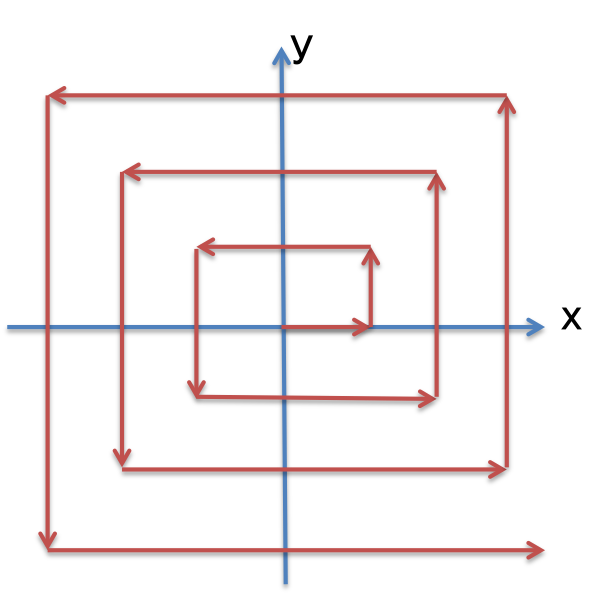
\includegraphics[clip,width=7.0cm]{fig1.png}
    \caption{}
    \label{fig:chokuseki}
  \end{center}
\end{figure}

\item
4と同様に、直積を順番に考え、今度は$(x,y)$の代わりに$\frac{x}{y}$として並べる。つまり\\
\[\frac{0}{0},\frac{1}{0},\frac{1}{1},\frac{0}{1},\frac{-1}{1},\frac{-1}{0},\frac{-1}{-1},\frac{0}{-1},
\frac{1}{-1},\frac{2}{-1},\frac{2}{0},\frac{2}{1},\frac{2}{2},\frac{1}{2},\frac{0}{2},\frac{-1}{2},\frac{-2}{2},\frac{-2}{1},\frac{-2}{0},\frac{-2}{-1},\frac{-2}{-2},\frac{-1}{-2},\frac{0}{-2},\dots\]
ここで、
\begin{enumerate}
\item 分母が0になっているものを削除。
\item 約分すると同じ値になるものは、後に出現しているものを削除。
\end{enumerate}
という操作をして、並べ直すと、
\[\frac{1}{1},\frac{0}{1},\frac{-1}{1},\frac{2}{-1},\frac{2}{1},\frac{1}{2},\frac{-1}{2},\dots\]
ここで、それぞれの分数の現れる順番と分数の値の関係は、自然数の集合から有理数全体の集合への全単射の写像になっている。よって、有理数全体の集合$\mathbb{Q}$は可算集合。
\item
ある集合$A$が可算集合とする。このとき、$A$の無限部分集合$X(X\subset A)$について考える。$A$は可算集合なので、自然数から$A$への全単射の写像$f:\mathbb{N}\to A$が存在する。ここで、$A$の集合を以下のように並べる。
\[f(1),f(2),f(3),f(4),\dots\]
さらに、この順番を保ちながら、$X$に含まれていない要素を取り除き、順番に番号を振る。この番号とそれぞれの要素の対応は、自然数の集合から$X$への全単射になっている。
\end{enumerate}
\end{document}

